\documentclass[10pt]{article}
\usepackage[margin=.7in]{geometry}\usepackage{amsmath,tikz,hyperref}
\setlength{\parindent}{0pt}\setlength{\parskip}{7pt}
\begin{document}
\textbf{Word traversal equals affine polynomial composition}\hfill2026-10-31\\T-1171. Producer proof; independent source-fidelity review pending.

The complete decoded output polynomial now satisfies
\[
 \operatorname{decodedPoly}(\operatorname{transform}(c,a,b,s))
   = C(s^{-1})\,f(aX+b).
\]
The proof identifies the exact ordered list of binomial contributions with the earlier symbolic outer-loop polynomial, matches every stored coefficient, and proves higher coefficients vanish. If the decoded scale satisfies $s=a^m$, the result equals the existing normalization map $T_m$.
\begin{center}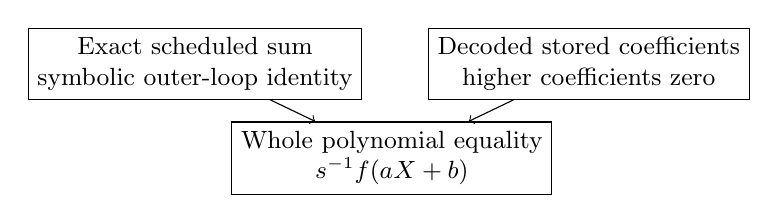
\begin{tikzpicture}[every node/.style={draw,align=center,font=\small}]
\node(a)at(0,0){Exact scheduled sum\\symbolic outer-loop identity};
\node(b)at(5,0){Decoded stored coefficients\\higher coefficients zero};
\node(c)at(2.5,-1.2){Whole polynomial equality\\$s^{-1}f(aX+b)$};
\draw[->](a)--(c);\draw[->](b)--(c);
\end{tikzpicture}\end{center}
The generic list/binomial identity allows arbitrary coefficient count over a field. The word-array theorem retains length $\le6$, prime $1<p<2^{31}$, canonical coefficients and parameters, and nonzero scale. The scale equality in the $T_m$ corollary is an explicit hypothesis.

Twelve main declarations and ten controls passed, with 22 named standard-axiom readbacks. Controls include empty/constant polynomials, identity at arbitrary length, a shifted/scaled quadratic, negative alpha, omitted scale, quintic leading coefficient and vanishing higher coefficients. For $f=1+2X+3X^2$ and $(a,b,s)=(2,3,4)$, the rational output coefficients are
\[
 [17/2,\;10,\;3].
\]
Changing $a$ to $-2$ changes the linear coefficient to $-10$; omitting the scale changes the constant coefficient. These are formal controls, not cohort measurements.

Identification attempt 1 required explicit list/function/coefficient rewrites. Attempts2--3 corrected a closed-goal tactic, notation parsed as a principal-segment token, and a conditional equality orientation. Attempt 4 passed. Reconstruction attempt 1 lacked an explicit prime-field instance; native exit 1 rejected it, including elaborator-generated sorry warnings. Attempt 2 passed; final named axiom readback contains no \texttt{sorryAx}. Controls and readback passed first attempt. All failures and nonfatal warnings are retained.

Sources: \texttt{projective\_law\_gate.rs} transform and the preceding loop, schedule, traversal, storage and arithmetic proofs. Primary reference: \href{https://leanprover-community.github.io/mathlib4_docs/Mathlib/Algebra/Polynomial/Coeff.html}{Mathlib polynomial coefficient identities}, through pinned imports.

Next source bindings: scale computation for the corollary, trailing-zero trimming and fixed-size divisor copying. This logical source model is not compiled-Rust equivalence or a geometric class transport proof. Existing compiled dependencies remain in the trust boundary. No scientific campaign, timing or cost ratio.
\end{document}
